\chapter{Transformer Architecture} \label{chapter:3}
Transformers \cite{attention_is_all_you_need} were proposed by Vaswani et al.\ in 2017. This novel architecture achieved state-of-the-art results in machine translation tasks, while dispensing with recurrent and convolutional architectures, which enabled parallelization and speedup of natural language processing tasks. The Transformer employs an encoder-decoder stack, each with multiple \emph{blocks}, as can be seen in Figure~\ref{fig:transformer}. The key mechanism behind this architecture is called \emph{attention}, which we will discuss in detail in a later section.

\begin{figure}[h]
    \centering
    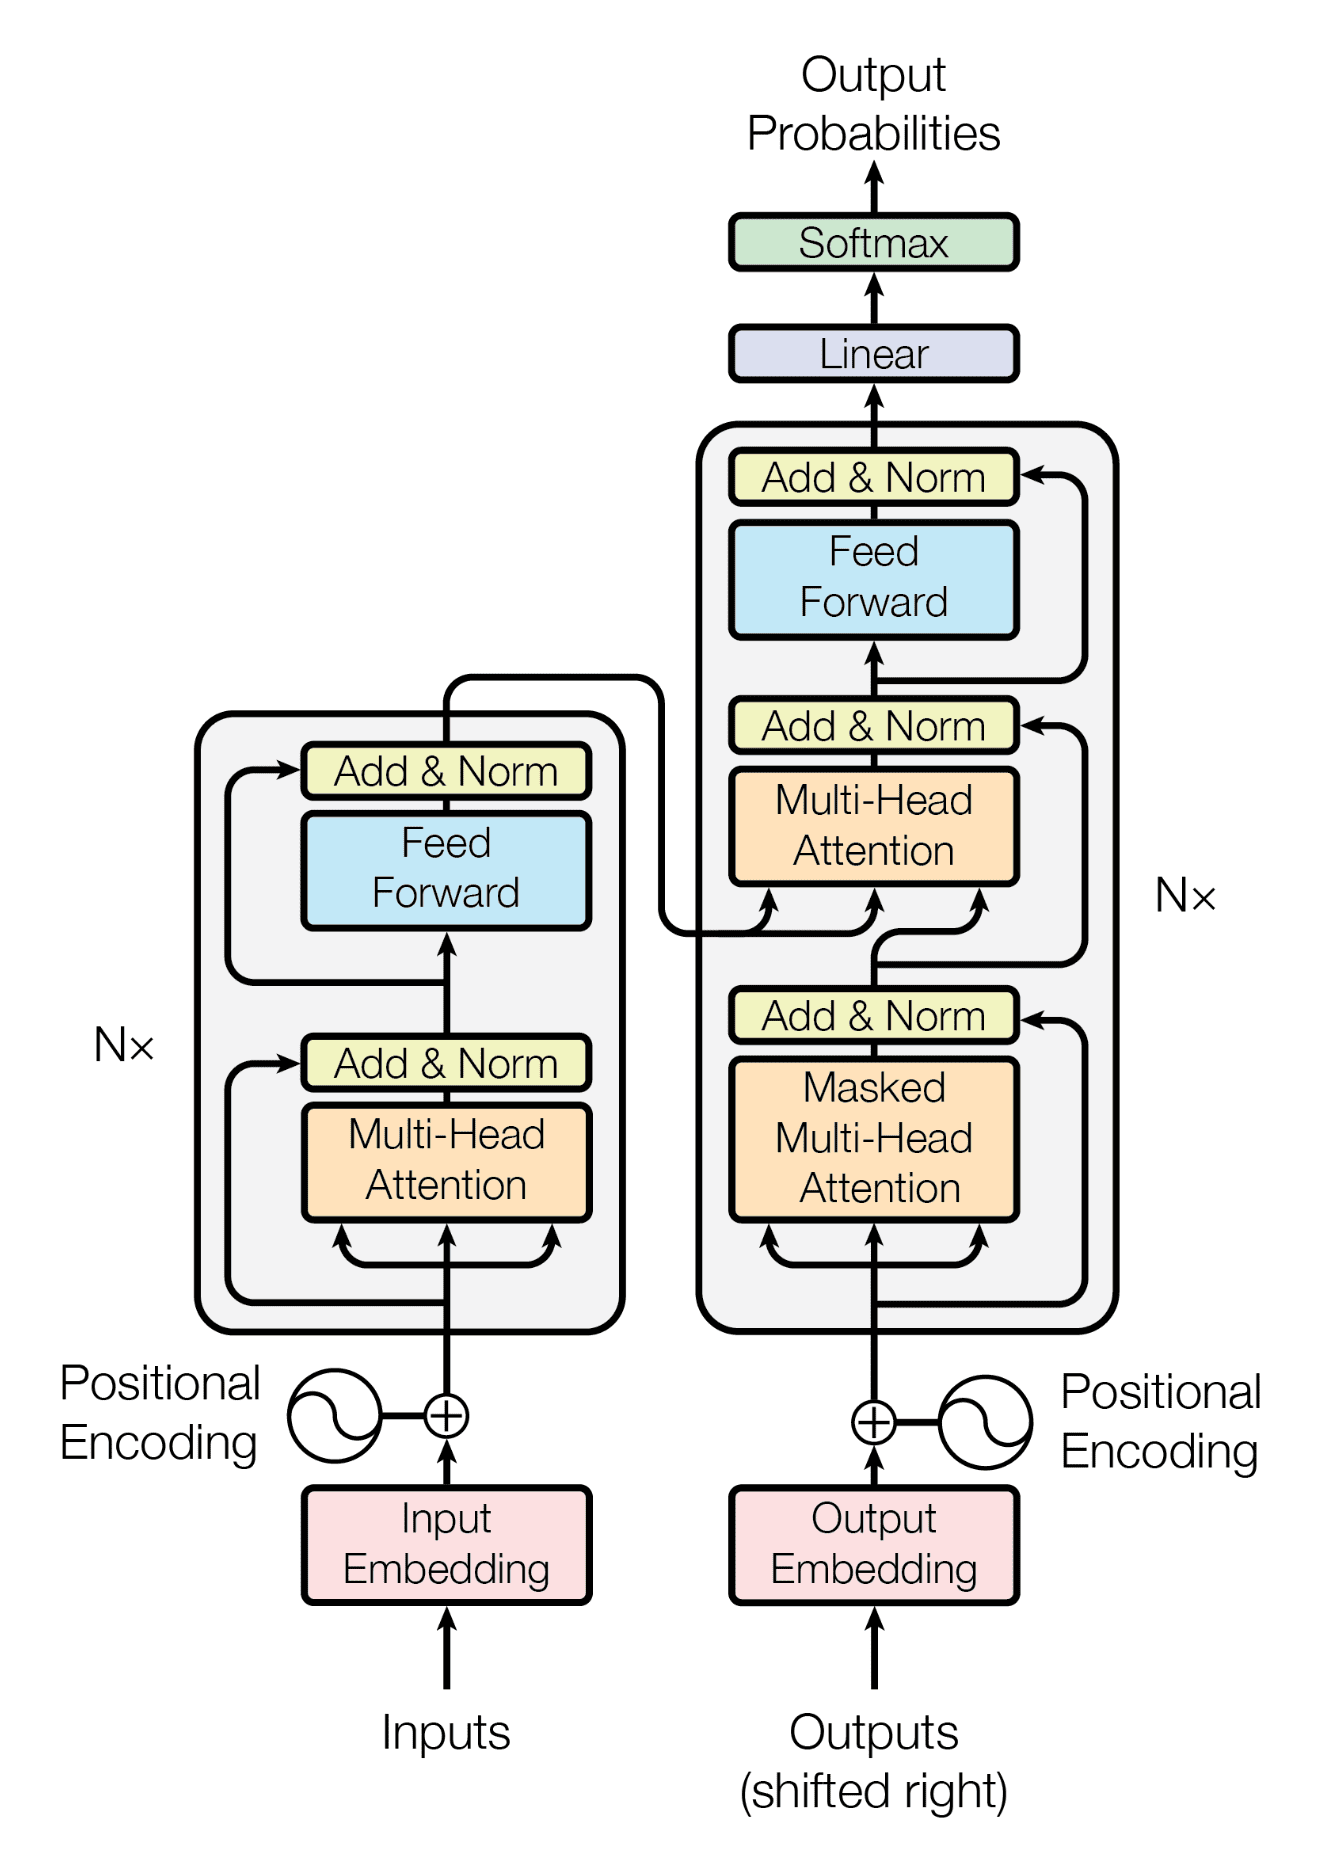
\includegraphics[width=0.6\linewidth]{figs/transformer.png}
    \caption{Transformer Architecture \cite{attention_is_all_you_need}}
    \label{fig:transformer}
\end{figure}

As we can see, the architecture lends itself to parallelization, since there are no recurrences or dependencies between inputs, which in turn helps speed up training and inference, but also increases the model's complexity and reduces its interpretability, due to the existence of residual paths, also called \emph{residual connections}, which are paths that add the input without processing to the output that stems from processing that same input, similar to doing $x = x + f(x)$ , layer normalizations and attention mechanisms.

For our work, we will focus on Transformer encoder stacks (which we will call encoder-only Transformers hereon forwards) with multi-head attention, as these can be used for sequence classification rather than machine translation or sequence modeling. In essence, Transformer encoder stacks map an input sequence $s \in \Sigma^*$ to a latent space $l \in (\mathbb{R}^{d})^*$.

Correspondingly, Transformer decoder stacks use this latent space, and an output start sequence and convert these inputs to a new sequence $s' \in \Sigma^{'*}$. This is a generative process, which we will not focus on.

These encoder-only Transformers, when used along a feed-forward layer and a softmax layer, use this latent space $l$ to output $n$-class classification probabilities, which we will use to determine if a string belongs to a certain language, after being trained on a dataset composed of strings of balanced and unbalanced parentheses.

\begin{figure}[h]
    \centering
    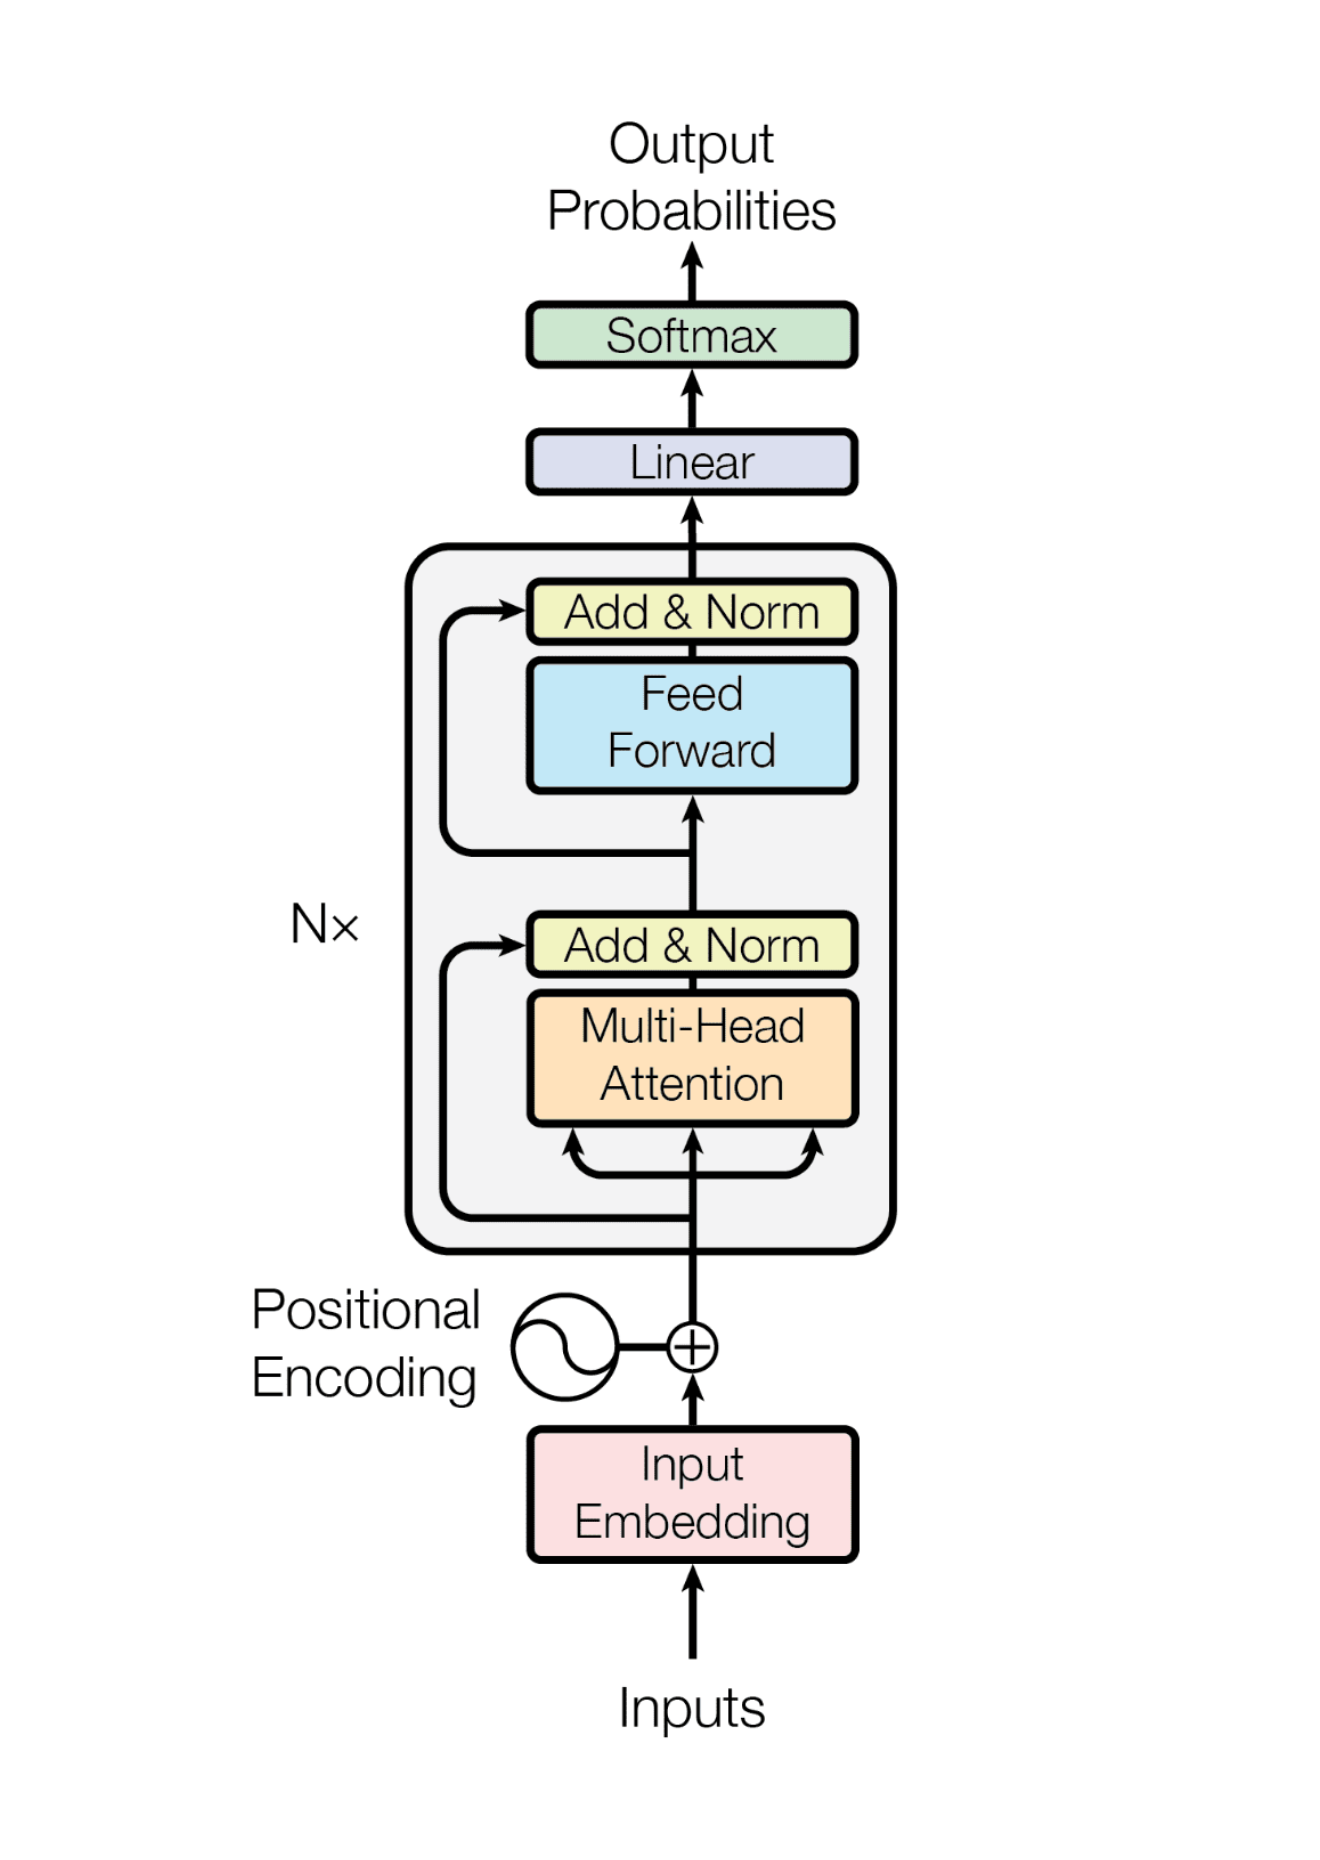
\includegraphics[width=0.6\linewidth]{docs/figs/transformer_classifier.png}
    \caption{Transformer classifier Architecture}
    \label{fig:transformer-classifier}
\end{figure}

Albeit Transformers are known for their state-of-the-art performance on natural language processing tasks, they cannot process words as-is; these inputs need to be mapped to a vector space $\mathbb{R}^d$. To this effect, we will use Ströbl's definition of a \emph{word embedding}, which is a length preserving function $\text{WE}: \Sigma \rightarrow \mathbb{R}^d$. This is part of the \emph{input layer}, which is defined in detail in Equation~\ref{eq:input_layer} \cite{strobl2024formal}. 

Figure \ref{fig:transformer} displays the full architecture of the original Transformer, with an encoder and decoder, each with its inner components, however, we will deal with a simplified version of this architecture, shown in Figure~\ref{fig:transformer-classifier}, and we will proceed to explain each part that makes up our encoder-only Transformers.

\section{Attention} \label{section:attention}
The attention mechanism is the most important part of this architecture and will be the focus of our study. In short, this mechanism will let the model know the importance of a \emph{token} with respect to all other tokens in the sequence.

This concept was introduced by Badhanau et al.\ and is defined as an alignment model \cite{badhanau-attn} that scores matches between inputs at a given position to outputs at another position. Even though this mechanism was applied to recurrent neural networks (RNNs), it is equivalent to the mechanism we will describe next.

According to Vaswani et al., attention functions can be described as mappings of queries and key-value pairs to an output, where queries, keys and values are all vectors belonging to a vector space $\mathbb{R}^d$, where $d$ is called the \emph{embedding} or \emph{representation} dimension. 

\paragraph{Input layer}
As mentioned previously, Ströbl defines these vectors as mappings that stem from applying a length preserving function, called the \emph{input layer}, $f: \Sigma^* \rightarrow (\mathbb{R}^d)^*$ to input strings\footnote{Ströbl et al.~use a different notation, $\Sigma^* \rightarrow (\mathbb{R}^d)^*$, compared to Vaswani et al., who represent these embeddings as $\mathbb{R}^{d\times n}$, to better align with conventions in formal language theory and emphasize variability in input sequence lengths.}. This function consists of two components, the previously defined word embedding and a positional encoding, PE, such that:

\begin{equation} \label{eq:input_layer}
    f(w_0\dots w_{n-1})_i = \text{WE}(w_i) +\text{PE}(i)
\end{equation}

\paragraph{Positional encoding}
A positional encoding (or embedding) is a function that maps the position of a token to our vector space $\mathbb{R}^d$. Formally,
\begin{equation} \label{eq:pos_enc}
    PE_{n}: |n| \rightarrow \mathbb{R}^d \text{ for } n \in \mathbb{N}
\end{equation}
where $|n| = \{0, 1, \dots, n-1 \}$~\cite{strobl2024formal}. We note 2 positional encodings of interest, absolute and sinusoidal.

Absolute positional encodings were defined by Yao et al.~\cite{bounded-hierarchical-languages} and are defined as follows: 
\begin{equation}\label{eq:abs_pos_enc}
    \text{PE}_{(i,n)} = \frac{i}{n}
\end{equation}
where $i$ is the token position and $n$ is the total token count (or length of the sequence).

Sinusoidal positional encodings were defined in Vaswani et al.~\cite{attention_is_all_you_need}, and are the seminal positional encoders for Transformers, defined as follows:

\begin{equation}\label{eq:sin_pos_enc}
    PE_{(pos, k)} =
    \begin{cases}
        \sin\left(\frac{pos}{10000^{\frac{k}{d_{model}}}}\right) & \text{if } k \text{ is even} \\
        \\
        \cos\left(\frac{pos}{10000^{\frac{k}{d_{model}}}}\right) & \text{if } k \text{ is odd}
    \end{cases}
\end{equation}
\\

\paragraph{Attention mechanism}
The most commonly used attention mechanism is called scaled dot-product attention or \emph{soft(max)} attention, which is defined as follows:

\begin{equation} \label{eq:attn}
    \text{Attention}(Q, K, V) = \text{softmax}\left( \frac{QK^T}{\sqrt{d_k}} \right)V
\end{equation}

In practice, $Q, K, V$ in equation \ref{eq:attn} refer to batched queries, keys and values respectively, where individual queries, keys and values are packed into matrices and processed simultaneously, speeding up computation.

Furthermore, this mechanism can be split and parallelized, which is then known as \emph{multi-head attention}, and represented by the following equation:
\begin{equation} \label{eq:multihead-attn}
    \begin{split}
        \text{MultiHead}(Q, K, V) &= \text{Concat}(\text{head}_1, \dots, \text{head}_n)W^O \\
        \text{where head}_i &= \text{Attention}(QW_{i}^{Q}, KW_{i}^K, VW_{i}^V)
    \end{split}
\end{equation}

In this mechanism, $W_{i}^{\{Q, K, V\}}$ are learned parameter matrices. Splitting the attention mechanism into different \emph{heads} allows for attending to information at different positions using different representations, without incurring in severe computational cost penalties, as the reduced dimensionality of each head allows for a computational cost similar to single-head attention with full dimensionality \cite{attention_is_all_you_need}.

We can also define \emph{hard} attention, which we define with the following equation:
\begin{equation}
    \text{HardAttention}(Q, K, V) = \text{argmax}\left( \frac{QK^T}{\sqrt{d_k}}\right)V
\end{equation}
We also note the difference between leftmost-hard and average-hard attention mechanisms, as the former looks for the first element with the maximum value, whereas the latter averages these and allows them to share weight equally \cite{strobl2024formal}.

Finally, we introduce the concept of \emph{self-attention}, which is simply applying the mechanism to the input sequence, in essence, allowing us to see internal relations within the sequence \cite{attention_is_all_you_need}.

We find this mechanism (\emph{self-attention}) of interest to our work, as we believe it will provide information regarding if a certain string of parentheses is balanced, and therefore, information about its membership to a Dyck-$k$ language.

\section{Attention Masks} \label{section:attn_masks}
We define an attention mask as follows:
\begin{equation}
    \begin{cases}
         0 & \text{if condition is true}  \\
         -\infty & \text{otherwise}
    \end{cases}
\end{equation}
We define 2 conditions of interest: $i\leq j$ and $\text{tok}[i] \neq \texttt{[pad]}$.

The first condition allows the mechanism to attend \emph{only} to previous positions, such that the mechanism cannot get information on tokens it has not yet seen - we call this mechanism future or \emph{causal} masking.

The second condition allows for the attention mechanism to ``see'' the sequence as a whole, but considers only tokens that provide information, ignoring special $\texttt{[pad]}$ tokens, used to unify input sequence lengths - we call this pad-token or \emph{bidirectional} masking. This masking is well known in the field of Transformers, as it is used by Bidirectional Encoding Representations from Transformers or BERT \cite{bert}.

We will analyze in further detail whether different attention masks have an effect on trainability in a later chapter.
